\documentclass [10pt,a4paper]{article}
\usepackage[danish]{babel}
\usepackage{a4wide}
\usepackage[T1]{fontenc}
\usepackage[utf8x]{inputenc}
\usepackage{amsmath}
\usepackage{amsfonts}
\usepackage{fancyhdr}
\usepackage{ucs}
\usepackage{graphicx}
\usepackage{listings}
\usepackage{color}

\pagestyle{fancy}
\fancyhead[LO]{Philip Munksgaard}
\fancyhead[RO]{Maskinarkitektur: G-Opgave 1}
\fancyfoot[CO]{\thepage}


\title{G-Opgave 1}
\author{Michael Thulin, Philip Munksgaard}

\begin{document}
\maketitle

\section*{Implementering af 4-bit ALU}
\subsection*{Opbygning}
Vi har fulgt den i opgaveformulering anbefalede fremgangsmåde og er
startet med at implementere en 1-bit full adder, dernæst en 1-bit ALU
og til sidst en 4-bit ALU. \\
Vi valgte for enkelthedens skyld at lave en traditionel ripple carry
adder. Vi kunne have valgt at lave en mere kompliceret carry lookahead
adder, og hvis vi havde haft mere tid kunne det sikkert have været en
givtig øvelse.

\subsection*{1-bit full adder}
1-bit full adderent består af en carry-komponent og en
sum-komponent. Vi startede derfor med at implementere hver af disse
komponenter som delkredsløb i logisim, for derefter at sætte dem
sammen i en 1-bit  full adder. Da vi havde valgt ikke at lave en
carry lookahead adder var dette ganske simpelt.

\subsection*{1-bit ALU}
Igen valgte vi for nemhedens skyld at følge beskrivelsen i Appendix C,
hvorfor 1-bit ALUen var relativt simpel at implementere som
delkredsløb.

\subsection*{4-bit ALU}
For at kunne lave en 4-bit ALU, var vi nødt til at lave en komponent
som kunne detektere overflow. Vi valgte at bruge resultatet fra opgave
C.25, så vores overflow detector kontrollerer bare, at cin og cout i
ALU for den mest betydende bit ikke er det samme. \\

\begin{figure}[h!]
  \centering  
    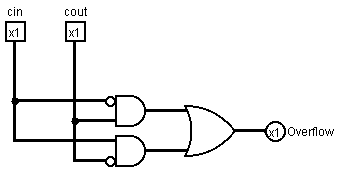
\includegraphics[scale=0.7]{overflow.png}
  \caption{Vores overflow-komponent.}
\end{figure}

\begin{figure}[h!]
  \centering  
    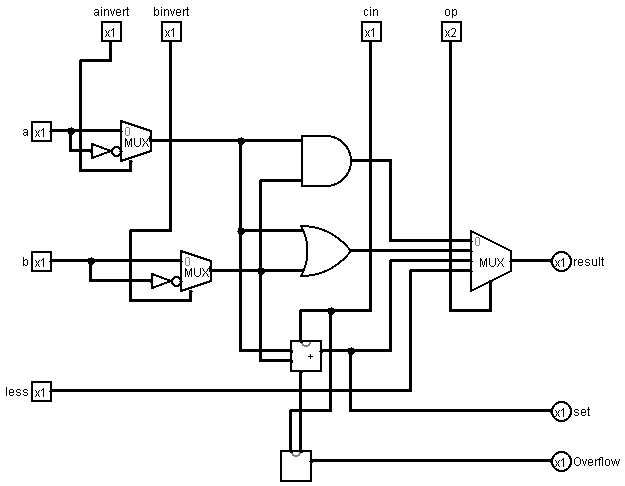
\includegraphics[scale=0.7]{ALUoverflow.png}
  \caption{Vores implementering af en 1-bit ALU med overflow detection.}
\end{figure}

\section*{Enkeltcyklusarkitektur}
Vi valgte at tage udgangspunkt i figur 4.17 i COD. Vi har desuden
valgt, ikke at bruge vores egen ALU, men den ALU der fulgte med
logisim.

\subsection*{16-32 bit sign extender}
Vi startede derfor med at implementere vores 16-32 sign
extender. Dette gjorde vi ved at tage den mest betydende bit i
input-værdien og kopiere den ud på de 16 mest betydende bits i
output-værdien.

\begin{figure}[h!]
  \centering  
    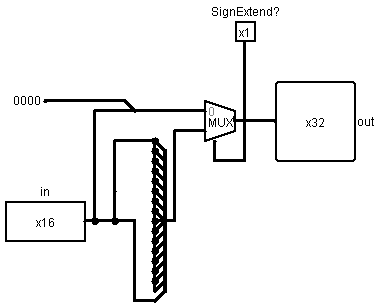
\includegraphics[scale=0.7]{bitextender.png}
  \caption{Implementering af 16-32 sign extender.}
\end{figure}

\subsection*{Control}
Vi har valgt at bruge PLAer til at understøtte vores sandhedstabeller
både i Control og i ALUControl. Dette gjorde det til en simpel opgave
at mappe OP-codes til Control-lines.\\
For at kunne understøtte immediate instruktioner valgte vi at lægge en
ekstra PLA ind i vores Control delkomponent, som kunne mappe OPcodes
til ALU operationer. \\
Af denne grund kunne vi simplificere vores ALUOp controllines, således
at alle R-instruktioner fik ALUOp 1 og resten af instruktionerne fik
ALUOp 0. Det vil altså sige, at vi har lavet en lille smule om i
forhold til implementationen i bogen.

\begin{figure}[h!]
  \centering  
    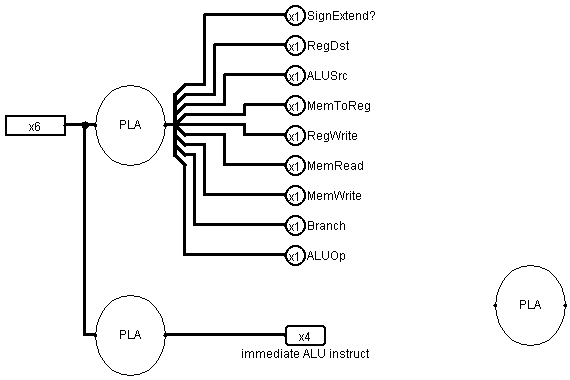
\includegraphics[scale=0.7]{control.png}
  \caption{Vores Control unit.}
\end{figure}

\subsection*{ALU Control}
Her har vi brugt en multiplexer, som vælger om ALU instruktionen skal
komme fra funct feltet i en R-instruktion, eller fra den ALU
instruktion vi genererer i Control-komponenten. Hvis ALUOp er 1 bruger
vi funct og hvis ikke bruger vi instruktionen fra Control.\\
Også her har vi valgt at bruge en PLA til at mappe fra funct til ALU
instruktion.

\begin{figure}[h!]
  \centering  
    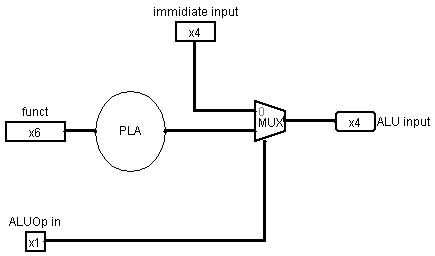
\includegraphics[scale=0.7]{ALUcontrol.png}
  \caption{Vores ALUControl komponent.}
\end{figure}

\subsection*{Test af MIPS-fortolker}
Vi har lavet 2-3 tests af hver MIPS-instruktion. Programmet test.asm
kan ses i bilag A. Alle instruktioner fungerer efter hensigten og
testen fejler ikke på noget tidspunkt.

\clearpage

\section*{Bilag A: Test af MIPS fortolker}
\lstinputlisting[language=Assembler]{test.asm}

\end{document}
